\documentclass{article}
\usepackage{arxiv}
\usepackage{iftex}
\ifPDFTeX\usepackage[utf8]{inputenc}\fi
\usepackage[T1]{fontenc}
\usepackage{amsmath,amssymb,booktabs,graphicx,microtype}
\usepackage[version=4]{mhchem}
\usepackage[numbers,sort&compress]{natbib}
\usepackage{url}
\usepackage{hyperref}
\usepackage{cleveref}
\usepackage{authblk}
\graphicspath{{figures/}}
\renewcommand{\thefigure}{S\arabic{figure}}
% Shared with main.tex and ijhmt/: the generated macros, tables and the bibliography.
% Generated from saved completed reports.
\newcommand{\BaselineCases}{15}
\newcommand{\FollowupCases}{64}
\newcommand{\ProductionCases}{19}
\newcommand{\TimeMin}{0.0043}
\newcommand{\TimeMax}{0.323}
\newcommand{\MeshMin}{2.06}
\newcommand{\MeshMax}{10.58}
\newcommand{\ProductionResidue}{1.41\times10^{-12}}
\newcommand{\SteelLLOne}{15.35}
\newcommand{\SteelLLTwo}{8.95}
\newcommand{\SteelLLThree}{1.98}
\newcommand{\SteelUpOne}{10.47}
\newcommand{\SteelUpTwo}{10.58}
\newcommand{\SteelUpThree}{2.13}
\newcommand{\PureLLOne}{5.70}
\newcommand{\PureLLTwo}{2.15}
\newcommand{\PureUpOne}{6.57}
\newcommand{\PureUpTwo}{5.06}
\newcommand{\SteelOrderOne}{1.3}
\newcommand{\SteelOrderTwo}{3.7}
\newcommand{\SteelErrApparent}{2.5}
\newcommand{\SteelErrSecond}{3.6}
\newcommand{\SteelSmoothThree}{0.67}
\newcommand{\SteelTotalThree}{0.015}
\newcommand{\SteelCentroidRange}{0.6}
\newcommand{\SteelCentroidTRange}{0.9}
\newcommand{\UpLLOne}{20.8}
\newcommand{\UpLLTwo}{14.1}
\newcommand{\UpLLThree}{11.3}
\newcommand{\UpLLFour}{7.7}
\newcommand{\PureUpLLMin}{9.0}
\newcommand{\PureUpLLMax}{13.2}
\newcommand{\VLSteelMax}{2.8}
\newcommand{\VLPureMax}{1.8}
\newcommand{\VLSteelThree}{1.16}
\newcommand{\VLPureThree}{0.27}
\newcommand{\IterPure}{1.09\times10^{-13}}
\newcommand{\IterSteelLow}{4.89\times10^{-13}}
\newcommand{\IterSteelHigh}{0.021}
\newcommand{\LobRMS}{18}
\newcommand{\LobRMSTemp}{35}
\newcommand{\LobRMSVap}{35}
\newcommand{\LobRMSGas}{17}
\newcommand{\LobCoarse}{0.2}
\newcommand{\LobDigitised}{1.0}
\newcommand{\LobFiveInlet}{548}
\newcommand{\LobFiveGas}{+3}
\newcommand{\LobFiveGasFraction}{4.0}
\newcommand{\LobLOneMin}{0.37}
\newcommand{\LobLOneMax}{0.89}
\newcommand{\LobRMSInlet}{135}
\newcommand{\LobFiveMain}{836}
\newcommand{\LobSixDeposit}{98.1}
\newcommand{\LobFiveUpstream}{1.2}
\newcommand{\LobShiftMin}{1}
\newcommand{\LobShiftMax}{4}
\newcommand{\LobCellsProd}{22{,}896}
\newcommand{\LobCellsCoarse}{10{,}176}
\newcommand{\GraetzBound}{1.69\times10^{-12}}
\newcommand{\GraetzRuns}{45}
\newcommand{\GraetzCriteria}{27}
\newcommand{\GraetzOrderHalfMin}{1.99}
\newcommand{\GraetzOrderHalfMax}{2.00}
\newcommand{\GraetzOrderNoneMin}{1.004}
\newcommand{\GraetzOrderNoneMax}{1.008}
\newcommand{\GraetzOrderSBHalf}{2.00--2.01}
\newcommand{\GraetzOrderSBNone}{1.01--1.02}
\newcommand{\GraetzGCIHalfMax}{1.89\times10^{-4}}
\newcommand{\GraetzGCINoneMin}{0.155}
\newcommand{\GraetzGCINoneMax}{0.341}
\newcommand{\GraetzExtHalfMax}{9.47\times10^{-9}}
\newcommand{\GraetzExtNoneMax}{1.10\times10^{-5}}
\newcommand{\GraetzMuH}{7.09\times10^{-9}}
\newcommand{\LobDiffA}{+26}
\newcommand{\LobDiffB}{+19}
\newcommand{\LobDiffC}{+16}
\newcommand{\LobDiffD}{$-$11}
\newcommand{\LobDiffE}{$-$14}

\newcommand{\vect}[1]{\mathbf{#1}}
\newcommand{\units}[1]{\,\mathrm{#1}}
\renewcommand{\thesection}{S\arabic{section}}
\renewcommand{\thetable}{S\arabic{table}}
\renewcommand{\theequation}{S\arabic{equation}}
\crefname{section}{Sec.}{Secs.}
\Crefname{section}{Section}{Sections}
\title{Supplementary material: Competition between radial diffusion and
interfacial exchange in thermal-gradient deposition columns}
\renewcommand\Authfont{\bfseries}
\setlength{\affilsep}{0em}
\author[1]{Jan Kren}
\author[1]{Bojan Ni\v{c}eno}
\affil[1]{Paul Scherrer Institute, 5232 Villigen PSI, Switzerland}
\date{14 October 2026}
\renewcommand{\shorttitle}{Supplementary material}
\renewcommand{\headeright}{Supplementary material}
\renewcommand{\undertitle}{Supplementary material to the working manuscript}
\hypersetup{colorlinks=true,linkcolor=blue,citecolor=blue,urlcolor=blue,
  pdftitle={Supplementary material: conservative modelling of iodine transport},
  pdfauthor={Jan Kren and Bojan Niceno}}
\begin{document}
\raggedbottom
\maketitle
\noindent This document collects the case inventory, the detailed
material-ledger and solver diagnostics, the scalar mesh checks of the
original upwind campaign, the comparison-bin-width analysis, the
property and thermodynamic records and the complete Graetz--Robin
verification table. Equations, tables and sections of the main text are
referred to by name. All numbers are generated from the same saved
results as the main text (\texttt{manuscript/prepare\_results.py},
\texttt{manuscript/assess\_resolution.py}).

\section{Case inventory}
\label{sec:s-cases}
\Cref{tab:study} lists the 64 follow-up cases of the original
18,432-cell upwind campaign. They cover the following cases:
\begin{itemize}
\item mesh and time-step checks: pure PbI$_2$ and three steel Q2 cases
  (baseline thermodynamics at 0.1\% and 1\% metal saturation, and
  shifted BiI thermodynamics at 1\%);
\item physical transport, accommodation, source-position and
  flow-reference variations: pure PbI$_2$, the two steel Q2 cases with
  baseline thermodynamics, and silica Q2 at 0.1\%;
\item extra source-loading cases: both columns and both thermodynamic
  branches;
\item temperature-coordinate variants: silica Q1 and silica Q2 at
  0.1\%.
\end{itemize}
This is a structured set of conditional comparisons, not a factorial
uncertainty study. Each numerical comparison changes one resolution
setting at a time.
\begin{table}[htbp]
\centering
\caption{Completed follow-up matrix: number of cases and the variation
applied in each study. The 15 baseline cases serve as additional
references. Flow-stop cases continue a 60 s baseline to 80 s.}
\label{tab:study}
\small\begin{tabular}{lrl}
\toprule
Study & Cases & Variation \\
\midrule
Mesh and time step & 12 & Three grids; 2 and 1 ms \\
Gas diffusion & 12 & $D/2$, $2D$, PbI$_2$--He correlation \\
Iodide accommodation & 8 & $\alpha=0.1$, 0.01 \\
Source position & 8 & $\Delta x_s=\pm1.5$ cm \\
Q2 metal loading & 12 & $\beta=0.002$, 0.003162, 0.005623 \\
Flow reference & 4 & 273.15 versus 298.15 K \\
Silica temperature coordinates & 4 & $\Delta x_T=-4.10$, $-4.65$ cm \\
Flow-stop relaxation & 4 & 60--80 s; fixed temperature \\
\bottomrule
\end{tabular}

\end{table}

The source-position alternatives move the release region by
$\pm1.5\units{cm}$ without adding a boat obstruction. The flow-stop
cases restart from the saved 60 s fields, remove injection, set the
carrier flow to zero and impose zero normal species flux at both ends.
The original nonuniform temperature profile stays fixed. These cases
therefore measure how residual gas redistributes during a 20 s flow
stop at fixed temperature; they are neither a clean-helium purge nor a
full cooling calculation.

\Cref{fig:physical} shows the largest baseline-relative iodine profile
change in each physical-input category of the main-text sensitivity
table.
\begin{figure}[htbp]
\centering
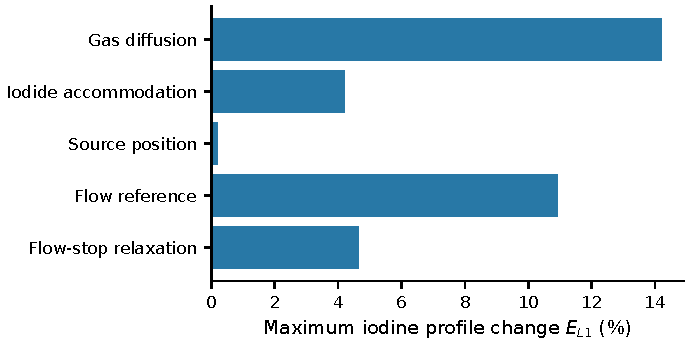
\includegraphics{physical_sensitivity.pdf}
\caption{Maximum baseline-relative iodine profile change $E_{L1}$ in
each selected physical-input category (upwind follow-up cases on
18,432 cells). The flow-stop value uses an 80 s endpoint; the others use
60 s. These maxima describe the tested case set, not a general
uncertainty budget or an experimentally identified parameter ranking.}
\label{fig:physical}
\end{figure}

Six further sets of runs complete the evidence, all with the same
solver executable. (i) The \ProductionCases{} production cases repeat
the 15 baselines and the four silica temperature-coordinate cases on
41,472 cells with the limited-linear scheme; all other inputs are
unchanged. (ii) A scheme and mesh study takes two cases, pure PbI$_2$
and the shifted-BiI steel case at 1\% metal saturation, which had the
largest upwind fine/medium change. It runs them with upwind,
limited-linear and van Leer advection on 8,192 to 41,472 cells, and the
steel case with upwind and limited-linear also on 93,312 cells. This
adds 12 runs to the existing upwind levels and the production runs.
Pure PbI$_2$ and the two unshifted steel Q2 cases were also run with
upwind on 93,312 cells, and a repeat of the shifted-BiI upwind run on
that mesh reproduced it bitwise.
(iii) Four original 18,432-cell upwind cases, the three baselines and
the shifted-BiI steel case at 1\% metal saturation, are repeated over
the full 60 s with eight instead of three species correctors. (iv) Ten runs
simulate five single-species PbI$_2$ experiments of Lobresco et al.\
\cite{Lobresco2026assessment} on two meshes. (v) The diffusivity
($D/2$, $2D$) and accommodation ($\alpha=0.1$, 0.01) variations of pure
PbI$_2$ and steel Q2 at 1\% metal saturation are repeated with the
production scheme on 41,472 cells (\PSRuns{} runs). (vi) \DaRuns{} runs
of a plane channel vary the accommodation coefficient over six decades
for the Damk\"ohler sweep of the main text, and \DaRefineRuns{} repeat
five of them with twice the wall-normal resolution. The stand-alone BiI$_3$
experiment at 800\,$^\circ$C was not run because its axial temperature
profile is not published.

\section{Material ledger and solver diagnostics}
\label{sec:s-ledger}
The frozen carrier keeps the converged face mass flux of the
\texttt{rhoSimpleFoam} solution rather than a flux reconstructed from
interpolated velocity. At these low mass flows, a zero-initialised
potential correction removes residual discrete divergence before species
transport. Carrier preparation rejects a carrier if its original cell or
global flux defect exceeds $10^{-6}$ of the inlet flow, or if a flux or
velocity correction exceeds $10^{-5}$ of the corresponding scale. After
correction, inlet, global and cell continuity and leakage through
impermeable boundaries are checked against $10^{-12}$ of the inlet flow.
This procedure is neither a new physical flow model nor evidence that
the velocity field has converged.

Element conservation is examined in two ways: through the solver
ledger and through the independently formed raw material residue of the
main text (Eq.~``balance''). The ledger also records the linear-solve
defect and any clamping correction separately. These terms explain
bookkeeping closure, but they are not inserted into the residue when
the raw material balance is assessed.

All residues are divided by the supplied material and taken as the
largest value over recorded steps and represented elements. The largest
raw residue is $\ProductionResidue$ for the 19 production cases
(41,472 cells, limited-linear advection) and $8.85\times10^{-13}$ for
the 60 source-driven follow-up cases; the 18,432-cell upwind baselines
had $5.97\times10^{-13}$. For the follow-up cases, the largest
accounted closure is $9.60\times10^{-16}$ and the largest recorded
solver defect is $8.64\times10^{-13}$; for the production cases they
are $1.12\times10^{-15}$ and $1.45\times10^{-12}$. The four flow-stop
cases keep their restart ledger and are excluded from this summary of
newly accumulated source material.

Canonical initialisation of the equilibrium solver makes a restarted
case independent of an unsaved equilibrium warm state. The baseline logs report no gas-equilibrium solver failures and a
maximum equilibrium element residue of $6.43\times10^{-16}$.
Input-validity and solver-success counters are distinct. At startup,
sign flags caused equilibrium to be skipped in up to 1,170 cells on
one step, and the maximum negative iodine diagnostic was
$1.14\times10^{-124}$ of supplied iodine. Matched five-step startup
replays identified extremely small leading-tail inventories at these
flags; no flagged cells remained at the final step. The calculations
should therefore not be described as free of negative trace values,
even though the reported amount is immaterial to the macroscopic
balance. The sum of the individual species mole-fraction maxima was at
most $9.19\times10^{-5}$. Because these maxima need not coincide, this
is an upper bound on the reactive trace loading, not a measured
mixture mole fraction at one location.

Some paired wall-coupling iterations did not meet the requested
$10^{-16}$ outer criterion. This is reported separately from
equilibrium failure, the final transport defect and the inventory-bound
checks. To test its effect, matched restarts of four representative
cases at 59 s compared three and eight correctors, and outer
tolerances of $10^{-16}$ and $10^{-14}$, over 20 time steps (40 ms).
The largest species-field change, scaled by its control maximum, was
below $3.6\times10^{-8}$, and the changes in new wall increments were
negligible. In the four full-run checks with eight correctors the
largest outer initial residual is still
$2.4\times10^{-15}$--$4.4\times10^{-15}$, and nearly every step ends at
the corrector limit, as with three: the requested $10^{-16}$ lies below
the attainable residual floor. No manufactured-solution test of the
full coupled system is presented; the Graetz--Robin test of the main
text verifies the wall discretisation only.

\section{Scalar mesh checks and binned maxima}
\label{sec:s-mesh}
Three-grid scalar checks follow the distinction between refinement
trends and an established asymptotic range
\cite{NASAGridConvergence,Roache1994perspective,Celik2008procedure}.
For the upwind follow-up triplets (8,192, 18,432 and 41,472 cells), 17
of the 34 nontrivial or zero-valued combinations of species, total,
centroid and width are oscillatory, four have nondecreasing
differences, one is unresolved at round-off and 12 admit only
conditional Richardson/GCI estimates. With upwind advection the
shifted-BiI steel case changes by essentially the same amount on the
first two refinements (\SteelUpOne\% and \SteelUpTwo\%). On 41,472
cells, van Leer and limited-linear advection differ by \VLSteelThree\%
(steel) and \VLPureThree\% (pure PbI$_2$).

With the production scheme (41,472 cells, limited-linear) the pure
PbI$_2$ binned maximum stays at 36 cm and 366.4--366.5\,$^\circ$C on all
three levels, and on 41,472 cells the 37 cm bin is 23\% lower; yet the
maximum of the 3 cm smoothed profile is at 37 cm and 350.5\,$^\circ$C,
and the wall temperature at the deposit centroid (37.11 cm) is
348.7\,$^\circ$C. In the upwind steel Q2 0.1\% case, the dominant
BiI$_3$ bin moves from 57 to 58 cm, and its reported temperature changes
from about 166.4 to 138.8\,$^\circ$C: a one-bin switch changes the peak
temperature by nearly 28 K without a comparable displacement of the
profile as a whole.

The local one-dimensional estimate $D_{\rm num}\simeq|u_x|\Delta x/2$
of the upwind numerical diffusion is a Taylor-series screening
estimate, not a measured truncation error for the radial,
variable-density coupled problem; it exceeds the prescribed
$10^{-4}\units{m^2\,s^{-1}}$ where $|u_x|$ exceeds 0.061 m/s on the
18,432-cell mesh.

\section{Dependence on comparison-bin width}
\label{sec:s-bins}
To distinguish sensitivity of the reported observable from a change in
the CFD mesh, the saved 1 cm iodine inventories of the original upwind
campaign were summed into groups of two and four consecutive bins.
Every possible integer-bin offset was tested for each width, retaining
partial end groups and the full deposited inventory. No CFD field was
recomputed and no sub-bin reconstruction was introduced.
\Cref{tab:bin-audit} gives the fine/medium inventory differences for
these coarser observables. Ranges reflect bin origin, not statistical
uncertainty.
\begin{table}[htbp]
\centering
\caption{Original upwind fine/medium iodine inventory-profile
differences (percent, 41,472 versus 18,432 cells) after aggregation of
native bins. The 2 and 4 cm ranges cover all respective integer-bin
offsets. $W_1$ uses the original 1 cm bin centres and separately
normalised profiles; it measures redistribution distance, not position
error against the experiment.}
\label{tab:bin-audit}
\small\begin{tabular}{lrrrr}
\toprule
Case & 1 cm & 2 cm & 4 cm & $W_1$ (cm) \\
\midrule
Pure PbI2 & 5.06 & 4.09--4.81 & 1.22--4.81 & 0.0610 \\
Steel Q2, 0.1\% & 5.26 & 1.77--4.12 & 0.51--2.45 & 0.0311 \\
Steel Q2, 1\% & 2.06 & 0.85--1.43 & 0.11--1.31 & 0.0115 \\
Steel Q2, shifted BiI & 10.58 & 3.37--10.02 & 0.52--10.02 & 0.0711 \\
\bottomrule
\end{tabular}

\end{table}

For the shifted-BiI case, a 4 cm comparison gives differences from
0.52\% to 10.02\% depending on the grouping origin, so a favourable
aggregation can hide a substantial local difference. Summing signed
bin differences before taking their absolute values necessarily allows
cancellation; a reduced aggregated L1 is not additional convergence
evidence.

As a complementary position-sensitive measure, let $p_b$ and $q_b$ be
the fine and medium iodine inventories normalised separately over the
whole column, and $x_b$ their common native bin centres. The
one-dimensional transport distance for these discrete distributions is
\begin{equation}
 W_1=\sum_{b=1}^{B-1}\left|\sum_{j=1}^{b}(p_j-q_j)\right|
                  (x_{b+1}-x_b).
 \label{eq:binned-wasserstein}
\end{equation}
It is the minimum mean distance needed to redistribute one normalised
binned inventory into the other. Values of 0.0115--0.0711 cm indicate
small average spatial redistribution between the two tested meshes,
despite larger local L1 differences. This is a distance between
computed binned profiles, not a bound on continuum error or evidence
that the experimental position uncertainty has been resolved. Four
analytical tests (edge-inventory preservation, signed-change
cancellation on aggregation, amplitude invariance of the shape measures
and a known point-mass displacement) check this post-processing, not
the CFD solver.

\section{Properties, thermodynamic provenance and units}
\label{app:properties}
This section lists the helium properties, molar masses, thermodynamic
records and optional PbI$_2$--He diffusivity used in the calculations.

\subsection{Helium and transported molecular masses}
The executed helium carrier uses
$M_{\rm He}=0.0040026\units{kg\,mol^{-1}}$,
$C_p=5193\units{J\,kg^{-1}\,K^{-1}}$ and
\begin{equation}
 \begin{gathered}
 \rho=\frac{pM_{\rm He}}{RT},\qquad
 \mu(T)=\frac{A_s\sqrt T}{1+T_s/T},\\
 A_s=1.4683\times10^{-6},\qquad T_s=83.40\units{K}.
 \end{gathered}
\end{equation}
The numerical value of $A_s$ gives viscosity in Pa\,s when $T$ is in K.
These are case inputs to the perfect-gas, constant-heat-capacity,
Sutherland model, not helium properties newly fitted to measurements.
Partial-pressure conversions use absolute pressure, while
thermodynamic activities use $p^\circ=10^5\units{Pa}$. The assumed
controller reference pressure, 101,325 Pa, is a separate quantity.
\Cref{tab:masses} lists the species masses used in transport and
stoichiometric conversion.
\begin{table}[htbp]
\centering
\caption{Molar masses of the nine transported gases. Condensed iodide
inventories use the same formula masses; the shared Pb and Bi
inventories use atomic masses.}
\label{tab:masses}
\begin{tabular}{lr@{\qquad}lr@{\qquad}lr}
\toprule
Gas & kg/mol & Gas & kg/mol & Gas & kg/mol \\
\midrule
Pb & 0.207200 & Bi & 0.2089804 & I & 0.12690447 \\
PbI & 0.33410447 & Bi$_2$ & 0.4179608 & I$_2$ & 0.25380894 \\
PbI$_2$ & 0.46100894 & BiI & 0.33588487 & BiI$_3$ & 0.58969381 \\
\bottomrule
\end{tabular}
\end{table}

\subsection{Thermodynamic records and phase treatment}
Pb--I--He functions are evaluated from external NASA nine-coefficient
records labelled with Gurvich source information. Bi--I functions use
an external ThermoFun compilation labelled HERACLES/Barin. A common
property evaluator converts all records to a consistent absolute
convention, $G^\circ(T)=H^\circ(T)-TS^\circ(T)$, before forming
reaction Gibbs energies. Mixing this convention with an apparent
formation Gibbs energy would give inconsistent equilibrium constants.
The solver tables store formation constants and phase-resolved vapour
pressures as logarithms. Input-file hashes, record identifiers and table-generation
scripts are recorded in the benchmark provenance.

For an iodide with one gas molecule per condensed formula unit,
\begin{equation}
 p_{\rm eq}(T)=p^\circ\exp\left[-\frac{G_g^\circ(T)
                                  -G_c^\circ(T)}{RT}\right],
 \label{eq:pv}
\end{equation}
evaluated on the stable available condensed branch. The BiI$_3$ liquid branch
is constructed at $T_{\rm fus}=680.85\units{K}$ from the crystalline
record with $\Delta H_{\rm fus}=31.798\units{kJ\,mol^{-1}}$ and
$C_{p,l}=150.624\units{J\,mol^{-1}\,K^{-1}}$, as recorded in the
input-generation metadata. It is a constructed phase record, not an
independently confirmed liquid thermodynamic dataset. Bi and
Bi$_2$ share condensed Bi but have different gas chemical potentials
and stoichiometry.

The BiI $+29$ kJ/mol variant modifies the gas record and regenerates
all formation and disproportionation constants consistently. Both the
baseline and the perturbed functions are hypotheses for the
sensitivity calculation; the BiI source record still needs independent
confirmation. The external coefficient files are not reproduced in the
manuscript data package. Numerical conservation of the model derived
from them cannot establish their physical correctness or complete the
provenance assessment.

\subsection{Optional \texorpdfstring{PbI$_2$}{PbI2}--He diffusion estimate}
Only the PbI$_2$--He transport variant uses the following implemented
correlation:
\begin{align}
 D_{\rm PbI_2-He}&=
 \frac{1.86\times10^{-7}T^{3/2}\sqrt{1/4.0026+1/461}}
 {(p/101325)\sigma^2\Omega(T^*)},\\
 T^*&=T/71.117857,\qquad \sigma=4.258468,\\
 \Omega(T^*)&=0.5313-1.2946e^{-0.9922T^*}\nonumber\\
             &\quad+\frac{1.5591}{T^*}-\frac{0.1918}{(T^*)^2}.
\end{align}
In this numerical expression $T$ is in K, $p$ in Pa, $\sigma$ in
\AA\ and the masses in g/mol; the resulting $D$ is in
$\mathrm{m^2\,s^{-1}}$. To reproduce the original correlation, the
implementation keeps 461 g/mol rather than the more precise transport
formula mass in \cref{tab:masses}. Its estimated collision parameters
follow the original polarisability/electron-count construction
recorded in the code. The other eight gases keep the constant baseline
coefficient in this variant. The correlation is a screening alternative,
not an experimentally validated binary diffusivity or a replacement
for all missing Pb--Bi--I transport data.


\section{Lobresco et al.\ comparison: set-up details}
\label{sec:s-lobresco}
The five cases of Lobresco et al.\ \cite{Lobresco2026assessment} are
computed on a 0.69 m, 5$^\circ$ wedge of 4.8 mm inner diameter whose
origin is taken to be the figure origin of that study (clean helium
enters at $x=0$ at the wall temperature there). The production mesh has
\LobCellsProd{} cells ($318\times72$), the axial and radial spacing of
the 41,472-cell Liu mesh, and the coarse mesh \LobCellsCoarse{} cells
($212\times48$), that of the 18,432-cell mesh. The time step is 2 ms,
0.5 ms at 540 mL/min. The sample is an evaporating inventory of the
Table 1 amount (times $5/360$ for the wedge), a cylinder 1 cm long and
0.48 mm in radius on the axis at the digitised sample arrow (0.13 m at
106 mL/min, 0.15 m at 5 and 540 mL/min); this geometry is an
assumption. The 106 mL/min wall temperature is the mean of the curves
of the T106\_6 and T106\_300 panels. Helium properties are those of the
Liu cases, not the NIST tables of that study. Carriers are audited to
$10^{-12}$ of the inflow; the largest absolute ledger closure over all
steps and runs is $3.3\times10^{-16}$ of the inventory.

A wall-temperature table distributed with the T-Flows test case of that
study differs from the published curves: its maximum of 1210 K lies at
0.04 m, whereas the figures peak at 1060--1070 K at 0.13--0.15 m, and
between 0.30 and 0.60 m it differs from them by up to 68--92 K. We use
the published curves.

\section{Graetz--Robin verification: all runs}
\label{sec:s-graetz}
\Cref{tab:graetz-full} lists every three-level sequence of the
Graetz--Robin verification ($\mathrm{Pe}_R=5$, \GraetzRuns{} runs including one
time-accurate control): Gauss linear advection with zero-gradient and
fixed-value outlets, and SuperBee advection, for both wall laws and
both Biot numbers. ``halfCell'' is the half-cell series law of the main
text and ``none'' the kinetic law applied to the cell-centre value. Every fitted decay rate equals that of the developed discrete mode of
the documented scheme within $\GraetzMuH$. Moving either or both ends
of the fit window by $\pm1.5R_t$, or fitting the mixing-cup concentration
or the wall uptake instead of the line density, changes $\kappa$ by less
than $10^{-7}$; the fixed-value outlet changes it by less than
$10^{-8}$. The reference error bound is $\GraetzBound$. On the
coarser 32/64/128 sequence the cell-centre law at Bi = 50 has
GCI$_{\rm fine}=0.678\%$; this triplet is too coarse for a first-order
wall law. The time-accurate control run ($N_r=32$, Bi = 50, half-cell
law, Courant number 1) reaches the decay rate of the discrete mode of
its mesh within $10^{-9}$. The records (reference, per-run fits,
criteria log and provenance, including the solver SHA-256) are in
\texttt{manuscript/data/graetz} with instructions to regenerate them.
\begin{table}[htbp]
\centering
\caption{Observed order $p$, relative error of the Richardson-extrapolated
decay rate and GCI$_{\rm fine}$ \cite{Celik2008procedure} (refinement
ratio 2, safety factor 1.25) for every three-level sequence of the
Graetz--Robin verification.}
\label{tab:graetz-full}
\small\begin{tabular}{lllllrrr}
\toprule
Scheme & Outlet & Bi & Wall law & $N_r$ & $p$ & $\kappa_{\rm ext}/\kappa_{\rm ref}-1$ & GCI (\%) \\
\midrule
linear & zeroGradient & 1 & halfCell & 32/64/128 & 2.0033 & $1.40\times10^{-8}$ & $7.55\times10^{-4}$ \\
linear & zeroGradient & 1 & halfCell & 64/128/256 & 2.0010 & $1.07\times10^{-9}$ & $1.89\times10^{-4}$ \\
linear & zeroGradient & 1 & none & 32/64/128 & 1.0154 & $3.50\times10^{-5}$ & $3.08\times10^{-1}$ \\
linear & zeroGradient & 1 & none & 64/128/256 & 1.0077 & $8.84\times10^{-6}$ & $1.55\times10^{-1}$ \\
linear & zeroGradient & 50 & halfCell & 32/64/128 & 1.9718 & $6.97\times10^{-8}$ & $4.06\times10^{-4}$ \\
linear & zeroGradient & 50 & halfCell & 64/128/256 & 1.9919 & $9.47\times10^{-9}$ & $1.00\times10^{-4}$ \\
linear & zeroGradient & 50 & none & 32/64/128 & 1.0081 & $3.88\times10^{-5}$ & $6.78\times10^{-1}$ \\
linear & zeroGradient & 50 & none & 64/128/256 & 1.0045 & $1.10\times10^{-5}$ & $3.41\times10^{-1}$ \\
linear & fixedValue & 1 & halfCell & 32/64/128 & 2.0033 & $1.40\times10^{-8}$ & $7.55\times10^{-4}$ \\
linear & fixedValue & 1 & halfCell & 64/128/256 & 2.0010 & $1.09\times10^{-9}$ & $1.89\times10^{-4}$ \\
linear & fixedValue & 1 & none & 32/64/128 & 1.0154 & $3.50\times10^{-5}$ & $3.08\times10^{-1}$ \\
linear & fixedValue & 1 & none & 64/128/256 & 1.0077 & $8.84\times10^{-6}$ & $1.55\times10^{-1}$ \\
linear & fixedValue & 50 & halfCell & 32/64/128 & 1.9718 & $6.97\times10^{-8}$ & $4.06\times10^{-4}$ \\
linear & fixedValue & 50 & halfCell & 64/128/256 & 1.9919 & $9.63\times10^{-9}$ & $1.00\times10^{-4}$ \\
linear & fixedValue & 50 & none & 32/64/128 & 1.0081 & $3.88\times10^{-5}$ & $6.78\times10^{-1}$ \\
linear & fixedValue & 50 & none & 64/128/256 & 1.0045 & $1.10\times10^{-5}$ & $3.41\times10^{-1}$ \\
SuperBee & zeroGradient & 1 & halfCell & 64/128/256 & 2.0024 & $4.68\times10^{-9}$ & $4.23\times10^{-4}$ \\
SuperBee & zeroGradient & 1 & none & 64/128/256 & 1.0143 & $1.63\times10^{-5}$ & $1.54\times10^{-1}$ \\
SuperBee & zeroGradient & 50 & halfCell & 64/128/256 & 2.0104 & $6.44\times10^{-8}$ & $1.30\times10^{-3}$ \\
SuperBee & zeroGradient & 50 & none & 64/128/256 & 1.0231 & $5.77\times10^{-5}$ & $3.36\times10^{-1}$ \\
\bottomrule
\end{tabular}

\end{table}

\bibliographystyle{unsrtnat}
\begingroup
\small
\bibliography{references}
\endgroup
\end{document}
